\chapter{Deadlock}
\label{chap:deadlock}

Quando l'uso contemporaneo delle risorse da parte di più processi porta a una situazione in cui nessun processo può proseguire senza aver accesso a una risorsa, si verifica un \textit{deadlock}.\newline
Un classico esempio di \textit{deadlock} è quello di due processi devono acquisire due risorse per completare il loro lavoro. Se il processo A acquisisce la risorsa 1 e il processo B acquisisce la risorsa 2, entrambi i processi non possono proseguire perché ciascuno aspetta che l'altro rilasci la risorsa di cui ha bisogno. Generalizzando sono necessarie quattro condizioni affinché si verifichi un \textit{deadlock}:
\begin{enumerate}
    \item \textbf{Mutua esclusione}: almeno una risorsa deve essere assegnata in modo esclusivo a un processo. Se una risorsa è assegnata a un processo, nessun altro processo può accedervi.
    \item \textbf{\textit{Hold \& Wait}}: un processo che detiene almeno una risorsa sta aspettando di acquisire altre risorse.
    \item \textbf{Nessuna \textit{preemption}}: una risorsa non può essere forzatamente rimossa da un processo che la detiene. La risorsa può essere rilasciata solo volontariamente dal processo che la detiene.
    \item \textbf{Attesa circolare}: esiste un insieme di processi {P1, P2, ..., Pn} tali che P1 sta aspettando una risorsa detenuta da P2, P2 sta aspettando una risorsa detenuta da P3, ..., e Pn sta aspettando una risorsa detenuta da P1.
\end{enumerate}
Per analizzare come una risorsa viene allocata ai processi, è utile costruire un \texttt{RAG} (\textit{Resource Allocation Graph}), un grafo diretto in cui i nodi rappresentano processi e risorse. Le risorse sono rappresentate da cerchi, mentre i processi sono rappresentati da quadrati. Un arco diretto da un processo a una risorsa indica che il processo sta aspettando la risorsa, mentre un arco diretto da una risorsa a un processo indica che la risorsa è attualmente assegnata al processo. Se esiste un ciclo nel grafo, si verifica un \textit{deadlock}, se ci sono più istanze di una risorsa ed esiste un ciclo allora non è detto che ci sia un \textit{deadlock}.
\section{Prevenzione del deadlock}
    Abbiamo diverse strategie per prevenire il \textit{deadlock}:
    \begin{itemize}
        \item Prevenzione Statica
        \item Prevenzione Dinamica
        \item Rilevamento (\textit{Detection}) e Recupero (\textit{Recovery})
        \item Struzzo - Non preoccuparsi del \textit{deadlock}
    \end{itemize}
    \subsection{Prevenzione Statica}
        La prevenzione statica del \textit{deadlock} implica l'uso della scrittura di codice che eviti che si verifichi una delle quattro condizioni necessarie per il \textit{deadlock}.
        \subsubsection{Mutua esclusione} 
            Non è possibile evitare la mutua esclusione, poiché è una condizione necessaria per l'uso delle risorse.
        \subsubsection{\textit{Hold \& Wait}} 
            \paragraph{Soluzioni}
                Per evitare questa condizione, un processo deve acquisire tutte le risorse di cui ha bisogno prima di iniziare a eseguire. Inoltre un processo può acquisire una risorsa solo se non detiene già altre risorse.
            \paragraph{Problemi} Questo approccio può portare a un utilizzo inefficiente delle risorse e a un aumento del tempo di attesa.
        \subsubsection{No preemption}
            \paragraph{Soluzioni} 
                Per evitare questa condizione, un processo che richiedere una risorsa non disponibile deve rilasciare tutte le risorse che detiene, oppure può cedere la risorsa che detiene su richiesta di un altro processo.
            \paragraph{Problemi} 
                Questo approccio è fattibile solo per risorse digitali come CPU e memoria, ma non per risorse fisiche come stampanti o dischi.
        \subsubsection{Attesa circolare} 
            \paragraph{Soluzioni}
                Per evitare questa condizione, è possibile assegnare una priorità ad ogni risorsa, in modo che un processo possa acquisire solo risorse con priorità superiore a quelle già detenute. In questo modo si evita la formazione di cicli di attesa in quanto un processo non può acquisire una risorsa con priorità inferiore a quelle già detenute.
            \paragraph{Problemi}
                Solitamente è difficile definire una priorità per le risorse, e questo approccio può portare a un utilizzo inefficiente delle risorse.
    \subsection{Prevenzione Dinamica}
        Dato che la prevenzione statica del \textit{deadlock} può portare a un utilizzo inefficiente delle risorse, in quanto queste tecniche impostano dei vincoli rigidi sul modo in cui i processi possono acquisire le risorse, la prevenzione dinamica punta a basare la prevenzione del \textit{deadlock} sulla base delle richieste delle risorse da parte dei processi. In questo modo, i processi possono acquisire le risorse in modo più flessibile, evitando il \textit{deadlock} senza compromettere l'efficienza delle risorse.
        \paragraph{Prerequisito} 
            Per utilizzare la prevenzione dinamica del \textit{deadlock}, è necessario che il sistema operativo conosca a priori il caso peggiore, ovvero il numero massimo di risorse che ogni processo richiederà. 
        \subsubsection{Il mentenimento del \textit{safe state}}
            \paragraph{Definizione} 
                Lo stato di assegnazione delle risorse, calcolato come il numero di istanze di risorse disponibili e il numero di istanze di risorse assegnate a ciascun processo su le richieste massime, è definito \textit{safe state} se esiste una \textit{safe sequence} di processi.
            \paragraph{\textit{Safe sequence}}
                Una sequenza di processi ($P_1,\dots,P_n$) è definita \textit{safe sequence} se ogni processo $P_i$, le risorse che richiede $P_i$ possono essere soddisfatte usando le risorse disponibili e le risorse rilasciate dai processi $P_1,\dots,P_{i-1}$.\newline
                Se non esiste una \textit{safe sequence} di processi, il sistema è in uno stato non sicuro (\textit{unsafe state}) e si potrebbe verificare un \textit{deadlock}, ma non è garantito che si verifichi. 
        \subsubsection{La prevenzione}
            Per mantenere il sistema in uno stato sicuro, il sistema operativo attua degli algoritmi per decidere se una richiesta di risorse da parte di un processo può essere soddisfatta senza portare il sistema in uno stato non sicuro. Dunque ad ogni richiesta di risorse da parte di un processo, il sistema operativo attua questa verifica.
            \paragraph{Svantaggi} 
                La prevenzione dinamica del \textit{deadlock} porta comunque ad una riduzione dell'efficienza del sistema, poiché il sistema operativo deve eseguire calcoli complessi per determinare se una richiesta di risorse può essere soddisfatta senza portare il sistema in uno stato non sicuro. Inoltre, la prevenzione dinamica riduce l'uso delle risorse rispetto ad un non-uso della prevenzione del \textit{deadlock}, poiché i processi devono attendere che il sistema operativo calcoli se la richiesta di risorse può essere soddisfatta.
        \subsubsection{Implenentazione}
            L'implementazione viene effettuata solitamente tramite o l'uso del \texttt{RAG}, oppure tramite l'uso dell' ``algoritmo del banchiere''.
            \paragraph{Uso di \texttt{RAG}}
                L'algoritmo che prevede l'uso di un \texttt{RAG} funziona solo se si ha una istanza per ogni risorsa.\newline
                Il \texttt{RAG} viene esteso con archi di ``rivendicazione'', ovvero archi che rappresentano una ``possibilità di richiesta'' di una risorsa da parte di un processo, $P_i\rightarrow R_j$ se $P_i$ in futuro potrebbe richiedere $R_j$. Questo comporta che ogni processo quando viene creato deve dichiarare le risorse che potrebbe richiedere in futuro.\newline
                In un secondo momento, il sistema operativo allocherà la risorsa $R_j$ al processo $P_i$ se l'arco $R_j\rightarrow P_i$ non crei un ciclo nel grafo. Se si verifica un ciclo, il sistema operativo non assegnerà la risorsa al processo $P_i$ in quanto porterebbe il sistema in uno stato non sicuro. Se il grafo non ha cicli, il sistema operativo assegnerà la risorsa al processo $P_i$ e rimuoverà l'arco di rivendicazione $P_i\rightarrow R_j$.
            \paragraph{Algoritmo del banchiere}
                L'algoritmo del banchiere è un algoritmo meno efficiente rispetto all'uso del \texttt{RAG}, ma funziona con qualunque numero di istanze di risorse.\newline
                Ogni processo è un cliente che possono richiedere del credito dalla banca (ovvero il sistema operativo) ogni risorsa allocabile è vista come del denaro. Ovviamente il \texttt{SO} non permetterà a tutti i clienti di raggiungere il massimo limite personale contemporaneamente. Ciò infatti porterebbe ad una situazione di \textit{deadlock}.\newline
                Anche in questo algoritmo ogni processo dichiarare il numero massimo di risorse che andrà ad richiedere, ad ogni richiesta di allocazione si verifica se questa mantiene lo stato \textit{safe}. Per fare ciò si sfruttano due algoritmi differenti, uno per l'allocazione ed uno per la verifica dello stato.
                \begin{lstlisting}[language=C++, caption={Algoritmo del banchiere}, label={lst:banker}, basicstyle=\small]
int available[m]// numero di istanze di R_i disponibili
int max[n][m]   // matrice delle richieste massime
int alloc[n][m] // matrice delle risorse allocate
int need[n][m]  // matrice delle richieste residue 
                // (need[i][j] = max[i][j] - alloc[i][j])

void request(int req_vec[]){
    if(req_vec[i] > need[i][j])
        error("Richiesta maggiore del massimo richiesto");
    if(req_vec[i] > available[j])
        wait();
    available[] = available[] - req_vec[];
    alloc[i][] = alloc[i][] + req_vec[];
    need[i][] = need[i][] - req_vec[];
    if(!state_safe()){
        available[] = available[] + req_vec[];
        alloc[i][] = alloc[i][] - req_vec[];
        need[i][] = need[i][] + req_vec[];
        wait();
    }
}

bool state_safe(){
    int work[m] = available[];
    bool finish[n] = {false, false, ..., false};
    int i;
    while(finish != {true, true, ..., true}){
        // cerca P_i che non e' terminato
        // e che puo' terminare
        for(i=0; i<n && (finish[i] || need[i][] > work[]); i++);
        if(i == n) // non esiste P_i che puo' terminare
            return false; // non e' in uno stato sicuro
        work[] = work[] + alloc[i][]; // rilascia le risorse di P_i
        finish[i] = true; // P_i e' terminato
    }
    return true; // e' in uno stato sicuro
}
                \end{lstlisting}
                Notare come questo algoritmo sia molto dispendioso e che deve essere eseguito ogni volta che un processo richiede una risorsa.\footnote{Nota dell'autore: È utile imparare questo algoritmo a memoria, in quanto verrà richiesto in sede di esame.}
    \subsection{Rilevamento del \textit{deadlock} \& ripristino}
        Gli algoritmi di rilevamento del \textit{deadlock} sono progettati per rilevare la presenza di un \textit{deadlock} nel sistema e per ripristinare il sistema a uno stato sicuro. Questi algoritmi sono meno restrittivi rispetto alla prevenzione (statico o dinamico) e consentono ai processi di acquisire le risorse in modo più flessibile. Tuttavia, richiedono un monitoraggio costante del sistema per rilevare la presenza di un \textit{deadlock} ed eventualmente correggere la situazione, questi possono comportare un sovraccarico significativo.\newline
        Esistono due approcci principali per il rilevamento del \textit{deadlock}: il rilevamento basato su \texttt{RAG} di attesa e l'``algoritmo di rilevazione''.
        \subsubsection{Rilevamento basato su \texttt{RAG}}
            Anche in questo caso il \texttt{RAG} funziona solo se si ha una istanza per ogni risorsa. Il grafo di attesa è un grafo composto da soli processi, ogni arco nel grafo ($P_i\rightarrow P_j$) indica che il processo $P_i$ sta aspettando una risorsa detenuta dal processo $P_j$. Se esiste un ciclo nel grafo, si verifica un \textit{deadlock}. Il sistema operativo può utilizzare questo grafo per rilevare la presenza di un \textit{deadlock} e per determinare quali processi sono coinvolti nel \textit{deadlock}. Tuttavia, questo approccio richiede che il sistema operativo monitori costantemente il grafo
        \subsubsection{Algoritmo di rilevamento}
            L'algoritmo di rilevamento esplora ogni possibile sequenza di allocazione dei processi che ancora non hanno terminato, se la sequenza và a buon fine, allora non c'è \textit{deadlock} altrimenti potrebbe esserci.\newline
            L'algoritmo è il seguente:
            \begin{lstlisting}[language=C++, caption={Algoritmo di rilevamento}, label={lst:detect}, basicstyle=\small]
int available[m]// numero di istanze di R_i disponibili
int alloc[n][m] // matrice delle risorse allocate
int req_vec[n][m] // matrice delle richieste

void check(){
    int work[m] = available[]; // risorse disponibili
    bool finish = {false, false, ..., false}; // processi terminati
    bool found = true; // trovato un processo che puo' terminare
    while(found){
        found = false; // resetta la variabile
        for(int i=0; i<n && !found; i++){
            // cerca P_i che non e' terminato
            // e che puo' terminare
            if(!finish[i] && req_vec[i][] <= work[]){
                // Assumo che P_i possa terminare senza deadlock
                // dunque rilascia le risorse senza deadlock
                work[] = work[] + alloc[i][]; // rilascia le risorse di P_i
                finish[i] = true; // P_i terminera' senza problemi
                found = true; // trovato un processo che puo' terminare
            }
        }
    }
    // Se finish[i] == false, per uno o piu'  P_i
    // allora i processi P_i sono in deadlock
}
            \end{lstlisting}
        \subsubsection{Ripristino}
            Prima di procedere al ripristino del \textit{deadlock}, bisogna capire ogni quando eseguire l'algoritmo di rilevamento del \textit{deadlock}, solitamente questo viene fatto o dopo ogni richiesta, o dopo $N$ secondi, oppure quando l'uso della \texttt{CPU} scende sotto una soglia $T$ preimpostata. \newline
            Una volta che il \textit{deadlock} è stato rilevato, il sistema operativo deve decidere come ripristinare il sistema a uno stato sicuro, ci sono diversi approcci per il ripristino del \textit{deadlock}.
            \paragraph{Uccisione di processi}
                La soluzione più comune per il ripristino del \textit{deadlock} è quella di uccidere uno o più processi coinvolti nel \textit{deadlock}. Ci sono due approcci principali per uccidere i processi:
                \begin{itemize}
                    \item Uccidere tutti i processi coinvolti nel ciclo - Soluzione molto costosa e drastica, ma è la più semplice da implementare.
                    \item Uccidere selettivamente i processi coinvolti nel ciclo - Questa soluzione è più complessa da implementare, ma può essere più efficiente in termini di utilizzo delle risorse, ma non dal punto di uso in quanto deve essere ri-eseguita la rilevazione dopo ogni uccisione.
                \end{itemize}
            \paragraph{Rilascio di risorse}
                Un'altra soluzione per il ripristino del \textit{deadlock} è quella di rilasciare alcune risorse detenute dai processi coinvolti nel \textit{deadlock}. Questa soluzione presente un problema: i processi che vengono forzati a rilasciare le risorse potrebbero non essere in grado di completare il loro lavoro normalmente, portando a un aumento del tempo di attesa e a una riduzione dell'efficienza del sistema. Inoltre se in situazione di \textit{deadlock} rilascio sempre le risorse coinvolte in uno stesso processo, si potrebbe verificare una situazione di \textit{starvation}, per ovviare questo si deve tener conto dei \textit{rollback} effettuati in precedenza.
    \subsection{Conclusioni}   
        Concludendo possiamo riassumere le varie soluzioni al \textit{deadlock} del seguente diagramma:
        \begin{figure}[H]
            \centering
            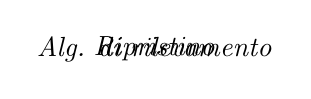
\begin{tikzpicture}
                \Tree [.Deadlock
                    [.{\textit{Prevenzione}} ]
                    [.{\textit{Evitare}} 
                        [.{\textit{DAG risorse}} ]
                        [.{\textit{Alg. banchiere}} ]
                    ]
                    [.{\textit{Rilevamento}} 
                        [.{\textit{DAG attesa}} [
                            .\node(R){\textit{Ripristino}}; 
                                [.{\textit{Uccisione processi}} ]
                                [.{\textit{Rilascio risorse}} ]
                            ]
                        ]
                        \node(Ri){\textit{Alg. di rilevamento}};
                    ]
                ]
            \draw (Ri) -- (R);
            \end{tikzpicture}
        \end{figure}

        Ognuno dei metodi ha i suoi vantaggi e svantaggi, e la scelta del metodo dipende dalle esigenze specifiche del sistema e dalle risorse disponibili. Principalmente però nessuno dei metodi di gestione è ottimale e delle soluzioni combinate di più metodi possono essere più efficaci se dividiamo le risorse in classi quali: risorse interne, memoria, risorse di processo (eg. file) e \textit{swap} applicando ad ognuna di queste la soluzione più efficiente: ordinamento di risorse per la prima, prelazione per la memoria, prevenzione dinamica per i file, e prevenzione con pre-allocazione (\textit{hold\&wait}) per la \textit{swap}.\newline
        In linea principale però la soluzione più semplice ed adottata dalla maggior parte dei \texttt{SO} è quella dello ``struzzo'' ovvero ignoriamo il problema del \textit{deadlock} in quanto si verificano raramente e tutte le soluzioni sono costose o con algoritmi sbagliati.